\subsection{Geographic dataset}
\label{section:geo_dataset}

%%%% generated by 2-time.py
\begin{figure*}[htp]
	\centering
	\begin{subfigure}[b]{0.35\textwidth}
		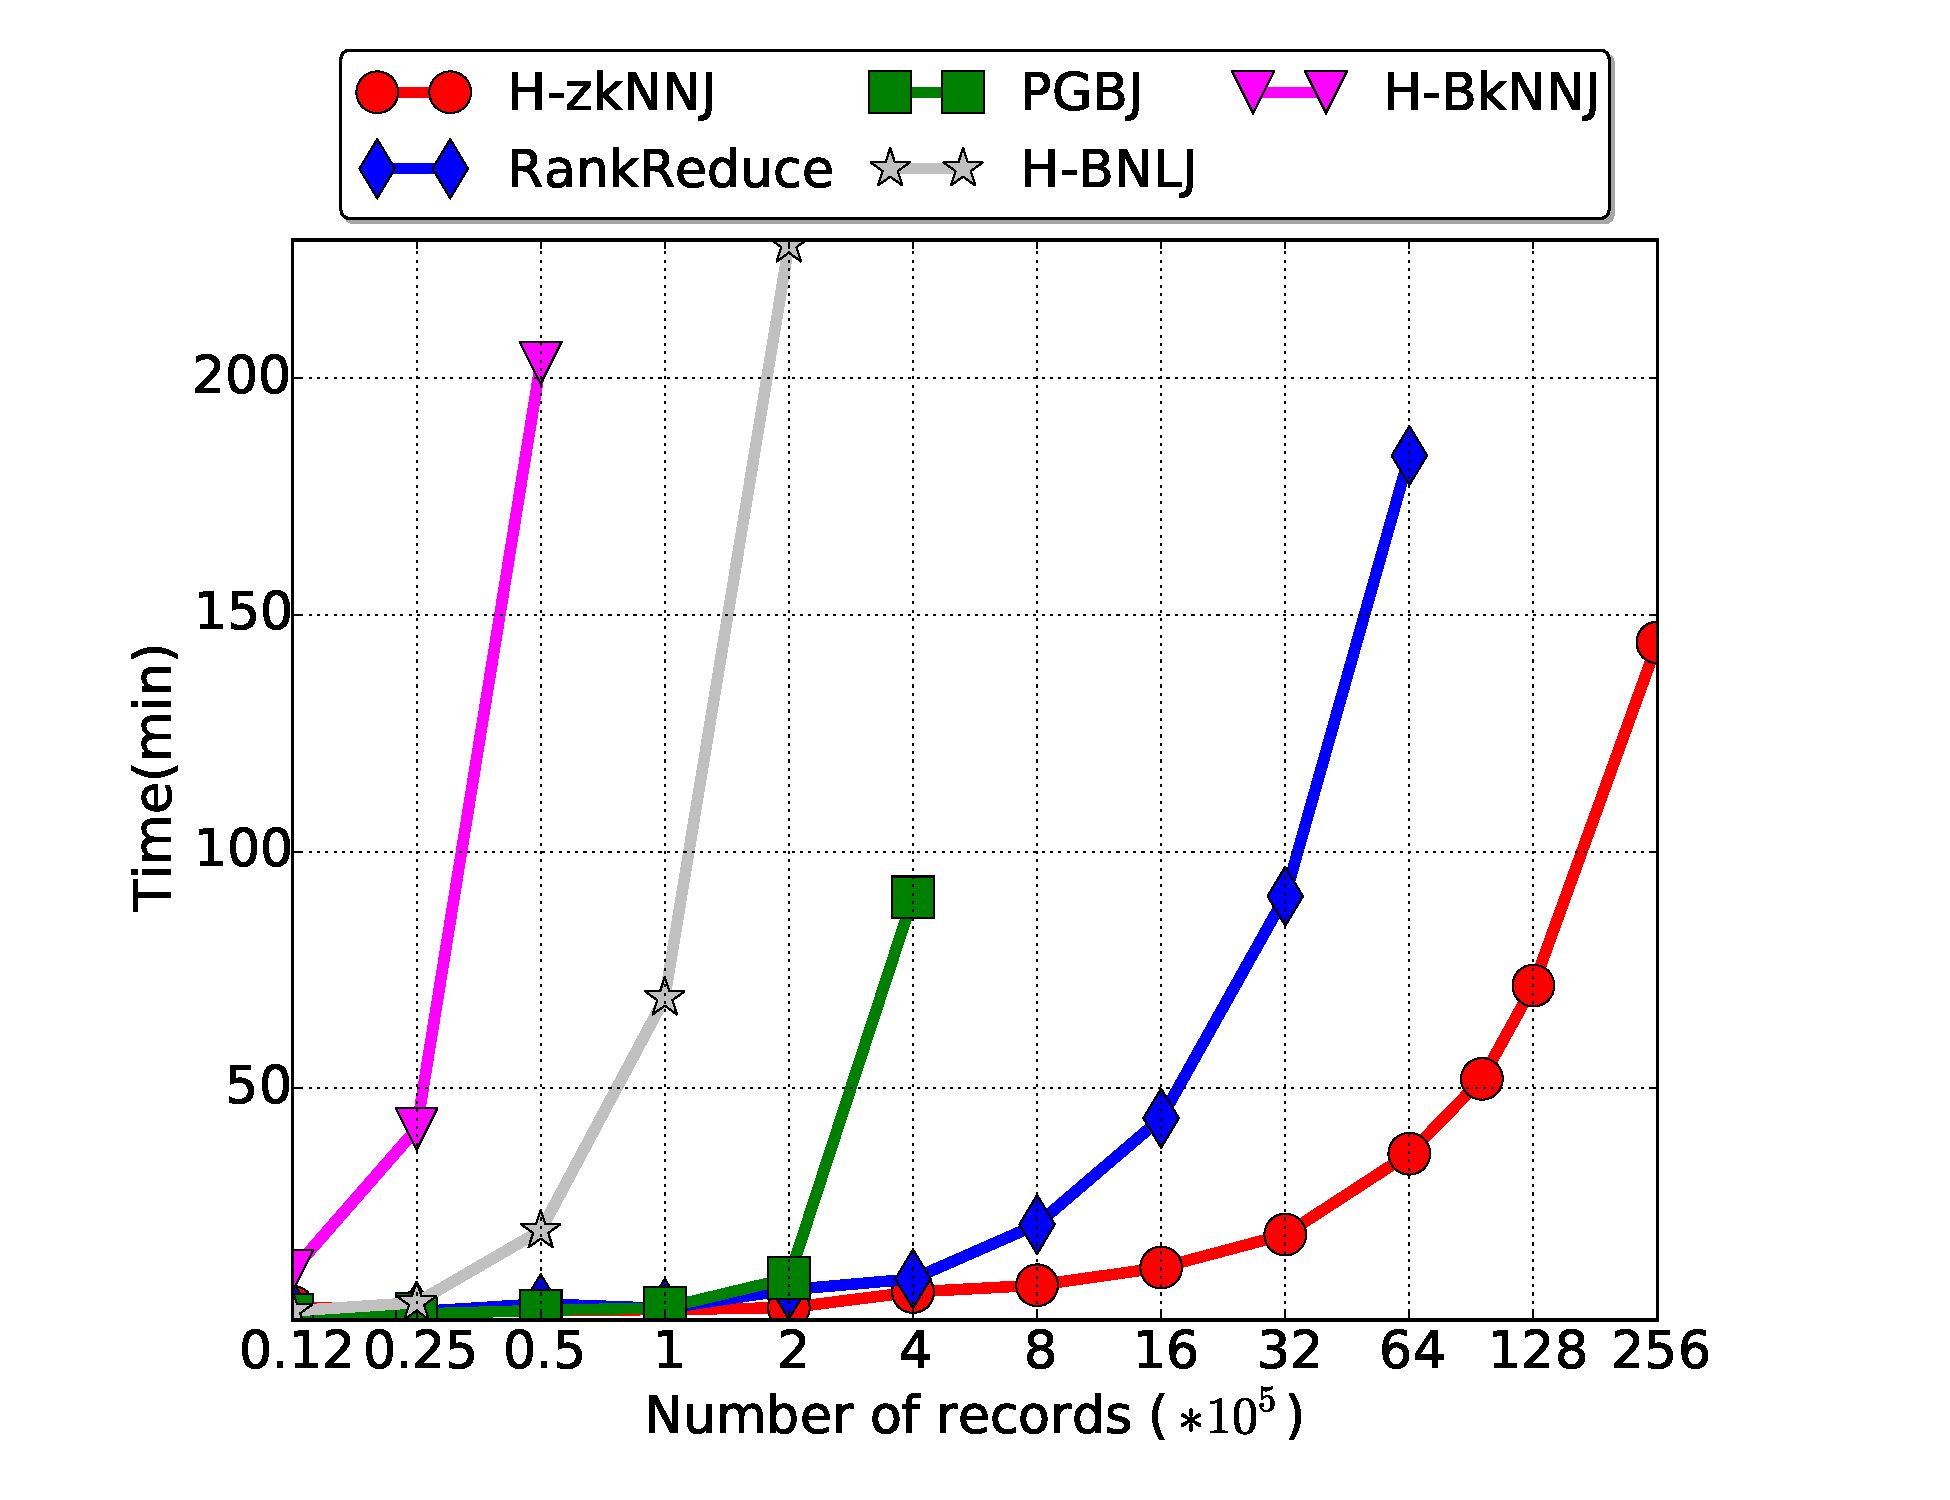
\includegraphics[width=\textwidth]{img-perf/geo/data/time.pdf} 
		\caption{Time}
		\label{fig:geo_data_time}
	\end{subfigure}%
	\begin{subfigure}[b]{0.35\textwidth}
		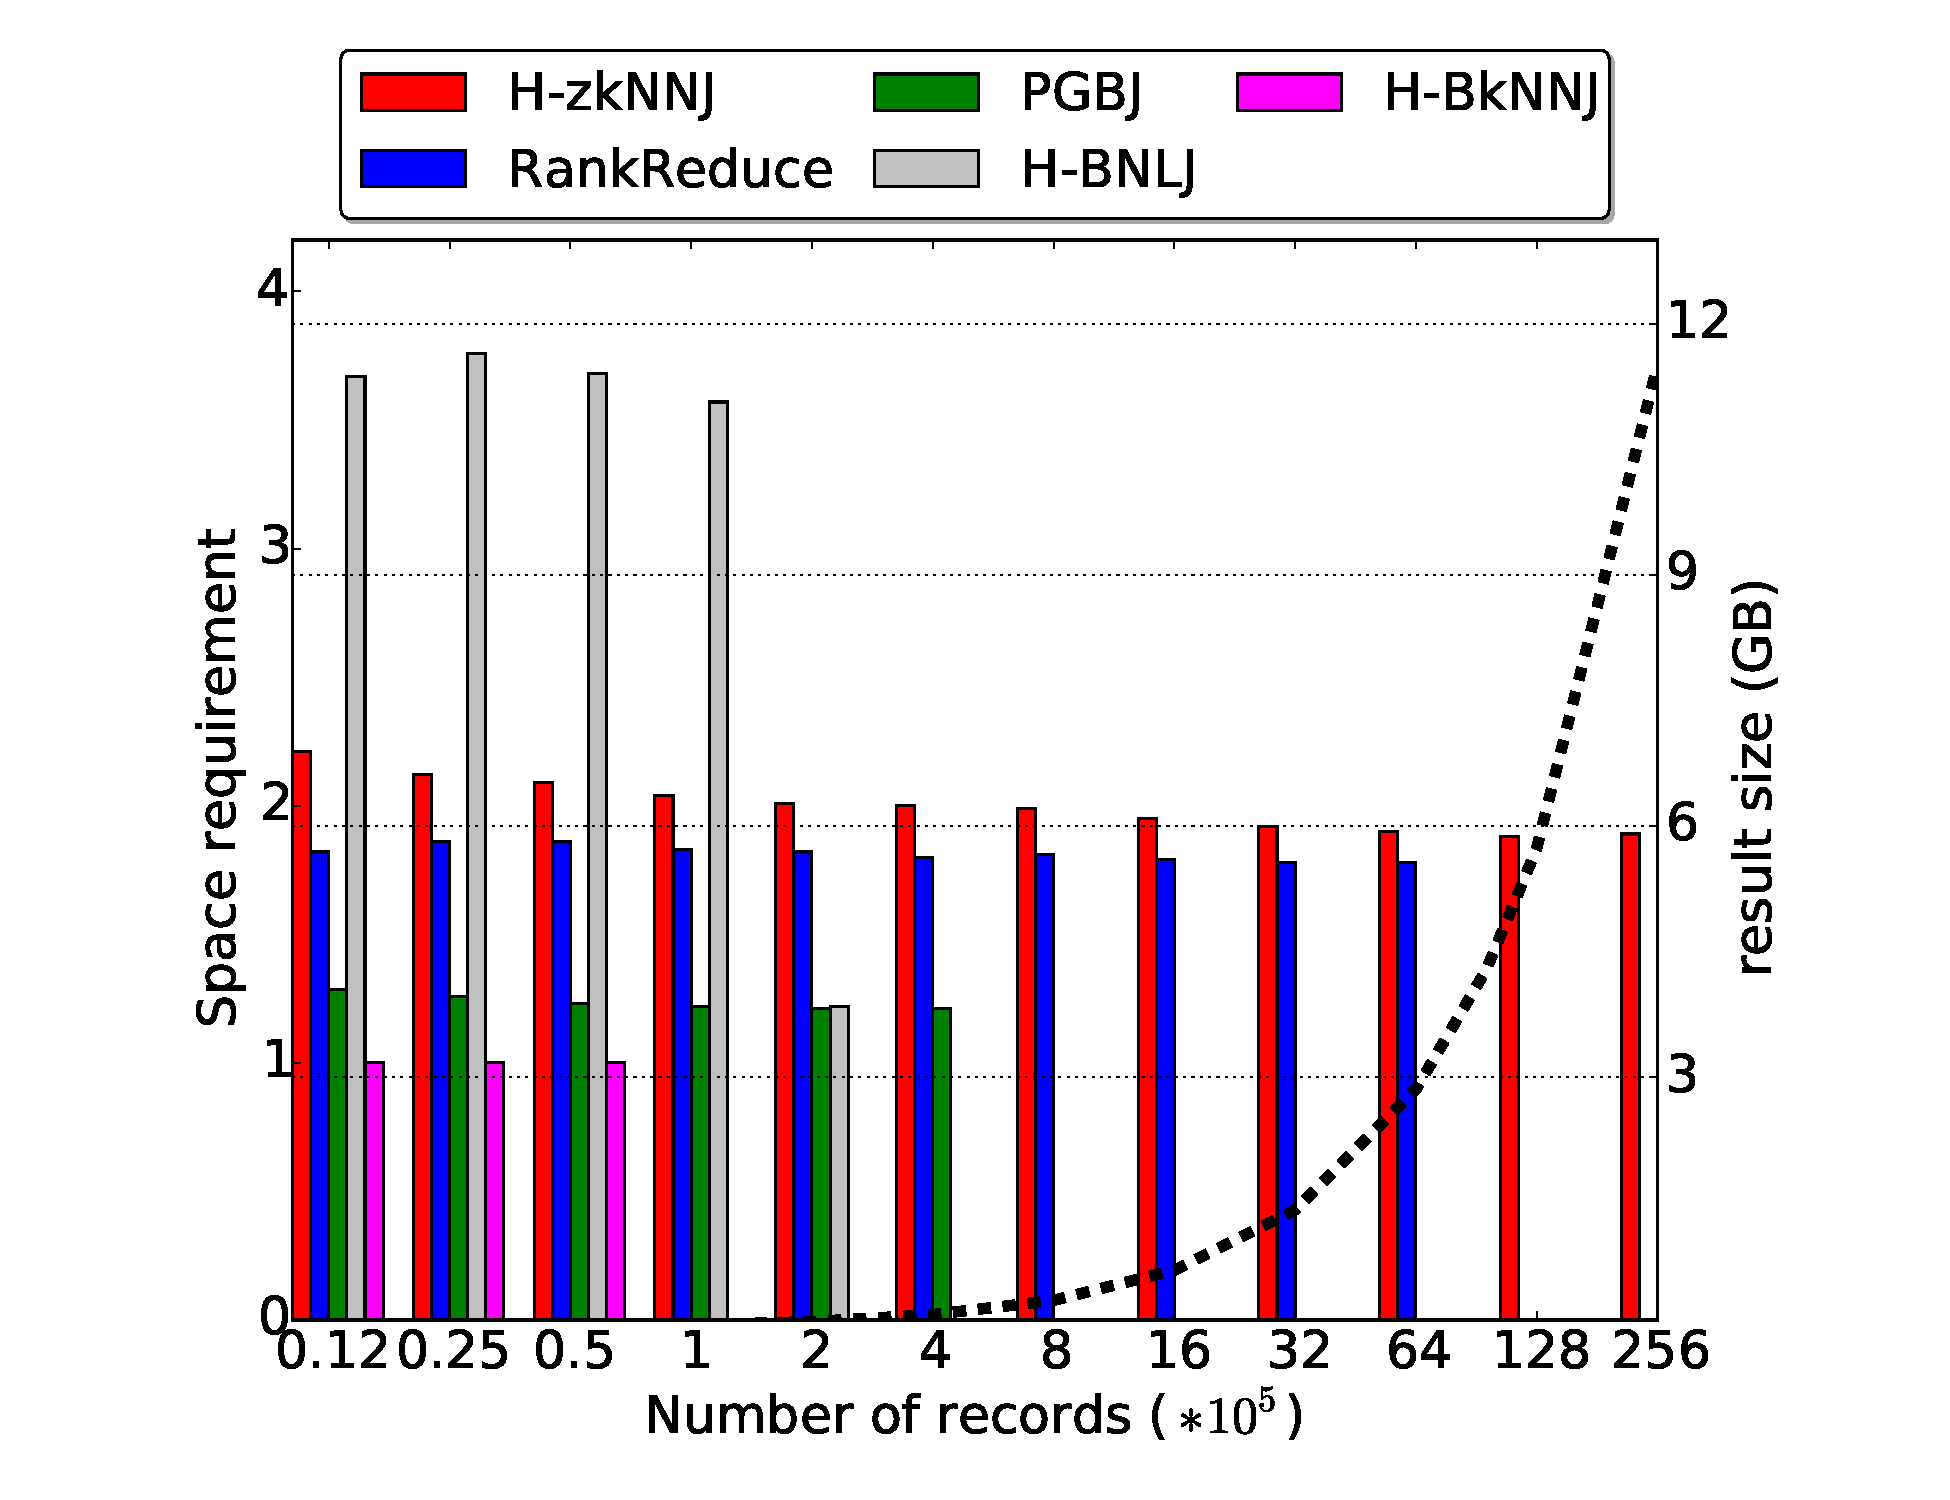
\includegraphics[width=\textwidth]{img-perf/geo/data/memory.pdf} 
		\caption{Result size and Disk Usage}
		\label{fig:geo_data_memory}
	\end{subfigure}%
	\begin{subfigure}[b]{0.35\textwidth}
		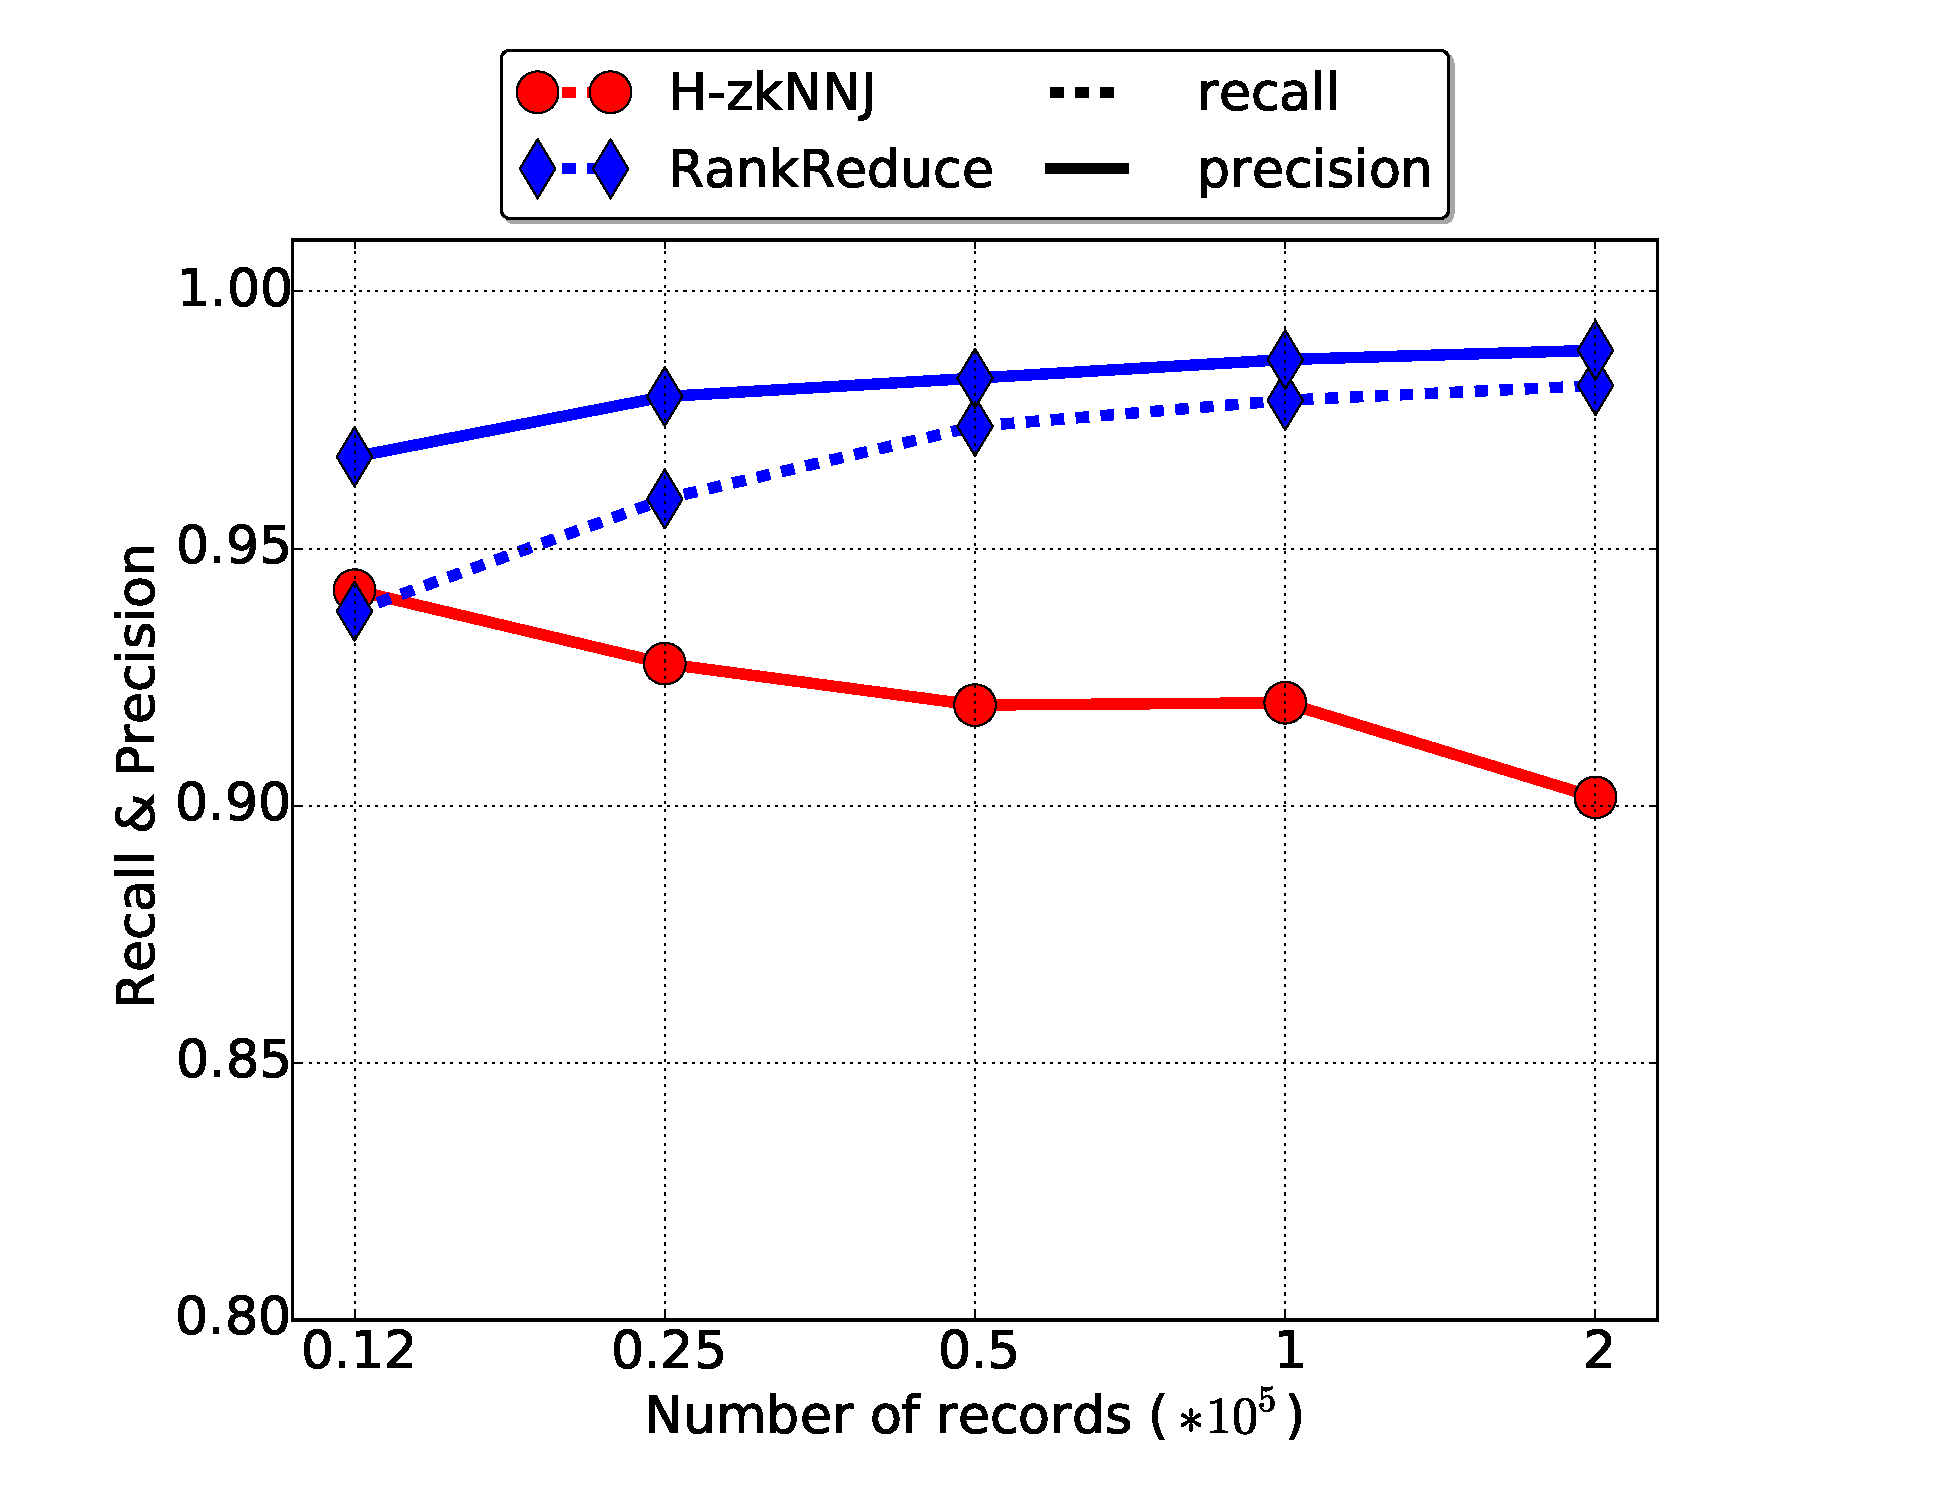
\includegraphics[width=\textwidth]{img-perf/geo/data/accuracy.pdf} 
		\caption{Recall and Precision \label{fig:geo_data_acc}}
	\end{subfigure}%
	\caption{Geo dataset impact of the data set size \label{geo_dataset}}
\end{figure*}


For all experiments in this section, we used the parameters described in Table~\ref{table:parameters_geo}.
Details regarding each parameter can be found in sections \ref{data_preprocessing} and  \ref{partitioning}. For 
RankReduce, the value of $W$ was adapted to get the best performance from each dataset. For datasets up to $16*10^5$
records, $W=32*10^{5}$, up to $25*10^{5}$ records, $W=25*10^{5}$ and finally, $W=15*10^{5}$ for the rest of the 
experiments. 

% shown in Table~\ref{table:parameters_geo}.
\begin{table}[ht]
\begin{center}{\renewcommand{\arraystretch}{1.2} % to prevent equation from being chopped 
\begin{tabular}{|c|c|c|c|}
\hline
\textbf{Algorithm} & \textbf{Partitioning} & \textbf{Reducers} & \textbf{Configuration}  \\ \hline
\HBNLJ             & 10 partitions  & 100 reducers & \\ \hline
\VO               & 3000 pivots     & 25 reducers       & \begin{tabular}[c]{@{}c@{}}k-means \\ + greedy\end{tabular} 
\\ \hline
\LSH          & $W = \left\{
\begin{array}{l}  
	32*10^{5}\\    
    25*10^{5}\\
	15*10^{5}\\
\end{array}\right.$
%$32*10^{5}$
% \TODO{this is plustot the size of bucket but not the number of partition. ??}           
& 25 reducers       & \begin{tabular}[c]{@{}c@{}}L = 2\\ M = 7\end{tabular}       \\ \hline
\Z~           & 10 partitions         & 30 reducers       & 3 shifts, 
p=10                                                     \\ \hline
\end{tabular}
}
\caption{Algorithm parameters \label{table:parameters_geo} for geographic dataset}
\end{center}
\end{table}


\subsubsection{Impact of input data size}
Our first set of experiments measures the impact of the data size on execution time, disk space and recall. 
Figure~\ref{fig:geo_data_time} shows the global computing time of all algorithms, varying 
the number of records from $0.125 * 10^{5}$ to $256 * 10^{5}$. The global computing time increases more or less 
exponentially for all algorithms, but only \Z~and \LSH~can process medium to large datasets. For 
small datasets, \VO~can compute an exact solution as fast as the other algorithms. 


Figure~\ref{fig:geo_data_memory} shows the space requirement of each algorithm as a function of the final output size. 
To 
reduce the footprint of each run, intermediate data are compressed. For example, for 
\HBNLJ, the size of intermediate data is $2.6$ times bigger than the size of output data. Overall, the algorithms with 
the
lowest space requirements are \LSH~and \VO.

Figure~\ref{fig:geo_data_acc} shows the recall and precision of the two approximate algorithms, \Z~and \LSH. Since \Z~
always return $k$ elements, its precision and recall are identical. 
As the number of records increases, its recall decreases, while still being high, because of the 
space filling curves used in the preprocessing phase.
On the other hand, the recall of \LSH~is always lower than its precision because it outputs less than $k$ elements. It
benefits from larger datasets because more data end up in the same bucket, increasing the 
number of candidates. Overall, the quality of \LSH~was found to be better than \Z~on the Geo dataset. 

%\input{parts/exp-dim-figure.tex}
\subsubsection{Impact of k}
Changing the value of $k$ can have a significant impact on the performance of some of the kNN 
algorithms. We experimented on a dataset of $2*10^5$ records (only $5*10^4$ for \HBNLJ~ 
for performance reasons) with values for $k$ varying from 2 to 512. Results are shown in 
Figure~\ref{fig:geo_impact_k} using a logarithmic scale on the x-axis.

First, we observe a global increase in computing time (Figure~\ref{fig:geo_k_time}) which matches the complexity 
analysis performed earlier. 
As $k$ increases, the performance of \Z, compared to the other advanced algorithms, decreases. This is due to the 
necessary replication of the $z$-values of $S$ throughout the partitions to find enough candidates: the core 
computation is thus much more complex. 

%%% generated by A4-ratioByK.py
\begin{figure*}[htp]
	\centering
	\begin{subfigure}[b]{0.35\textwidth}
		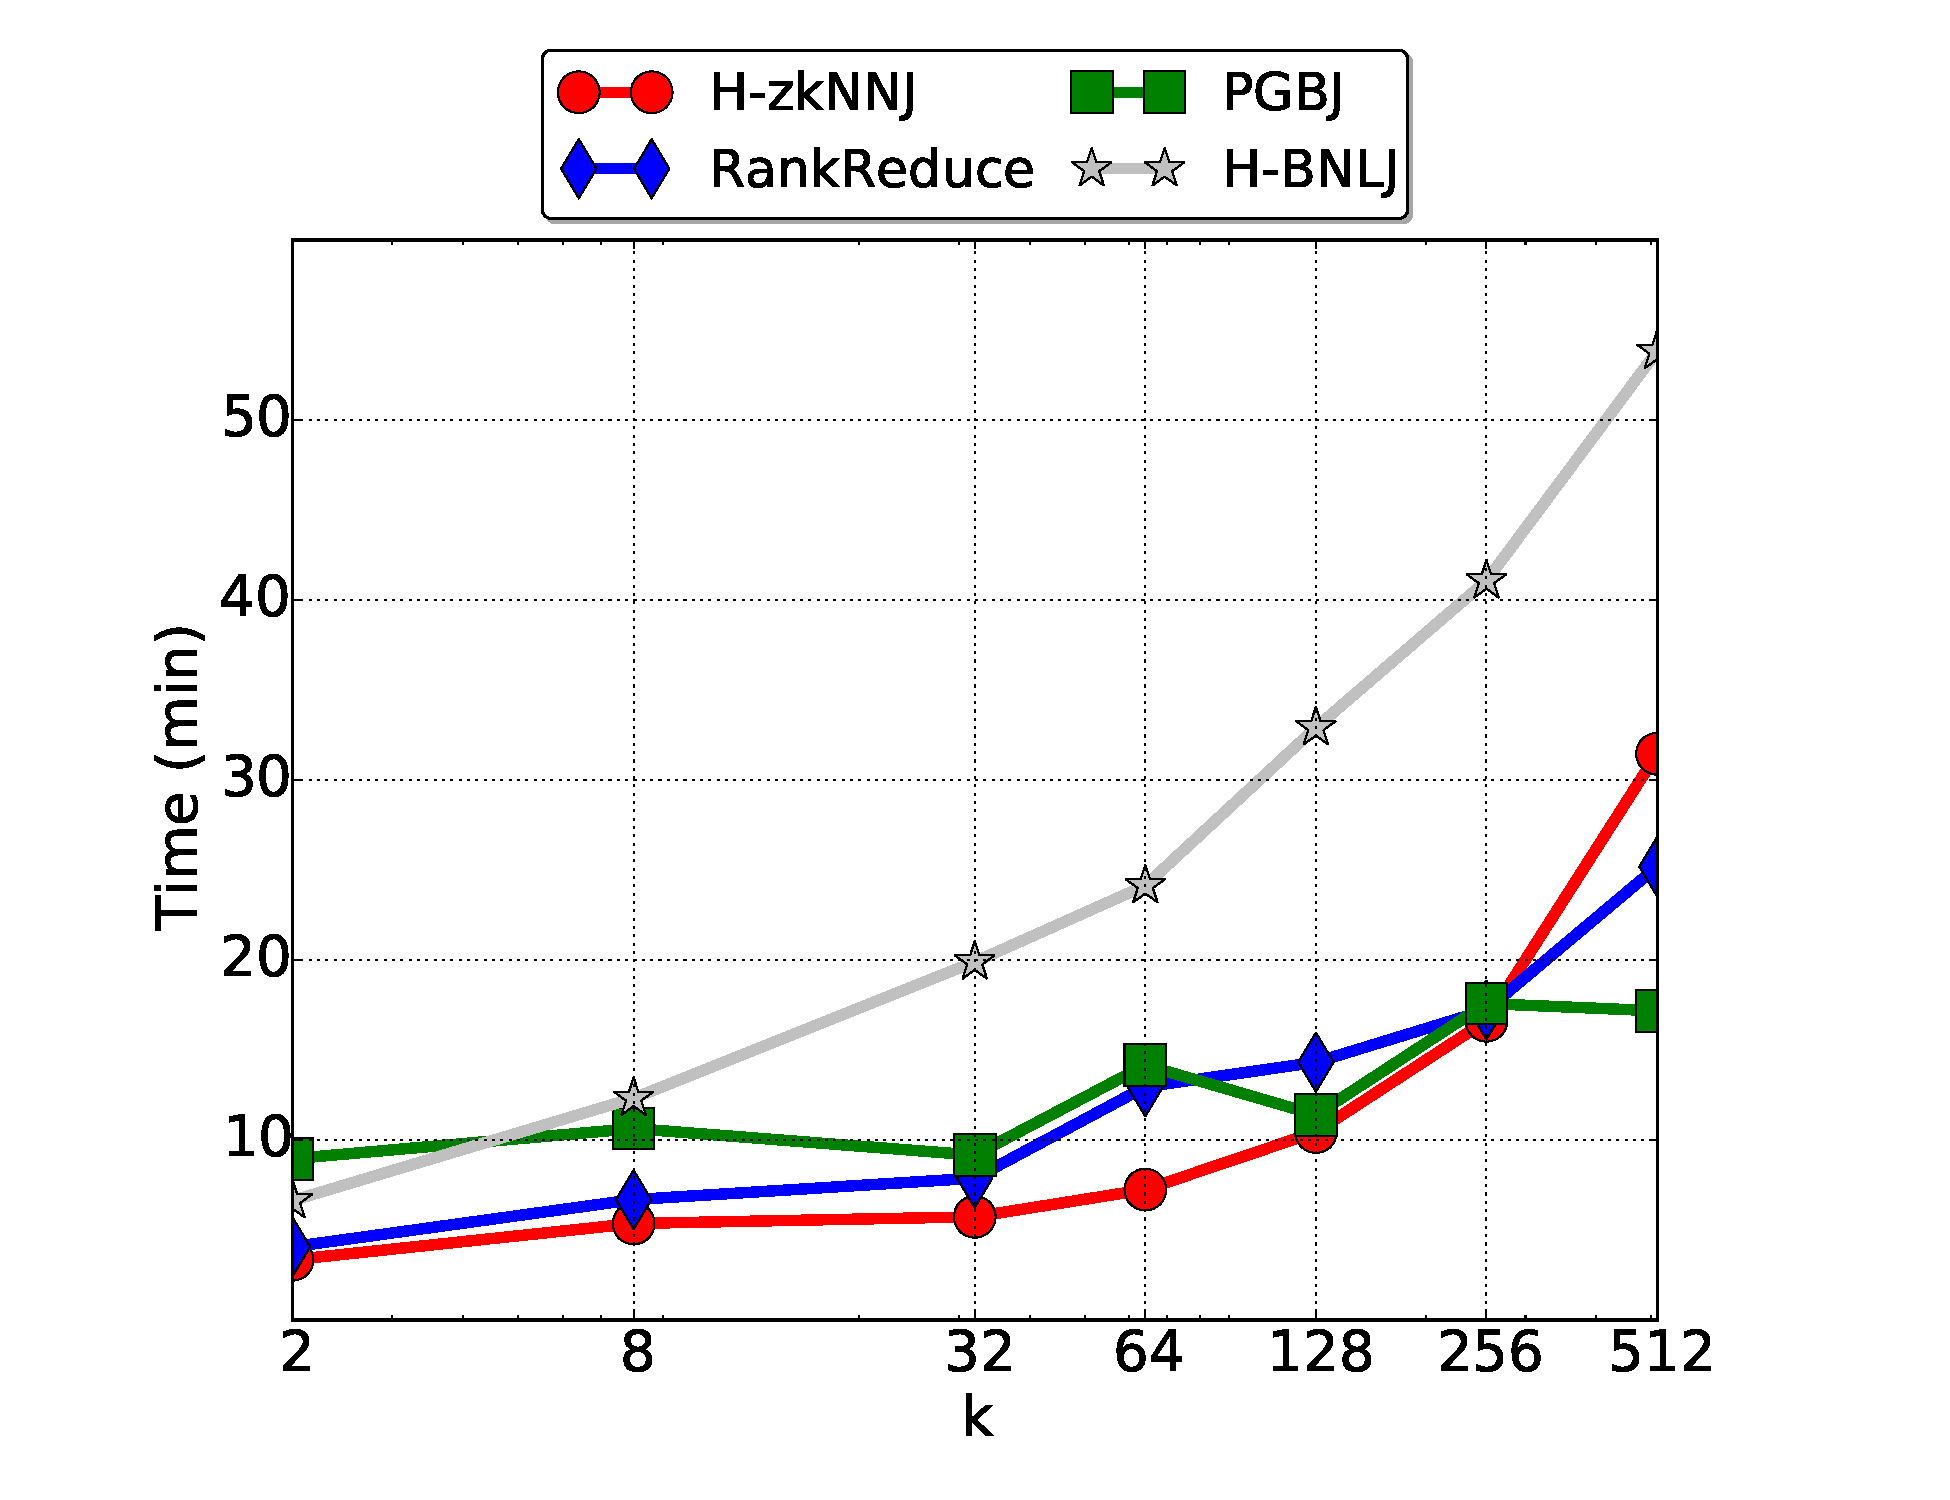
\includegraphics[width=\textwidth]{img-perf/geo/k/time.pdf} 
		\caption{Time\label{fig:geo_k_time}}       
	\end{subfigure}%
	\begin{subfigure}[b]{0.35\textwidth}
		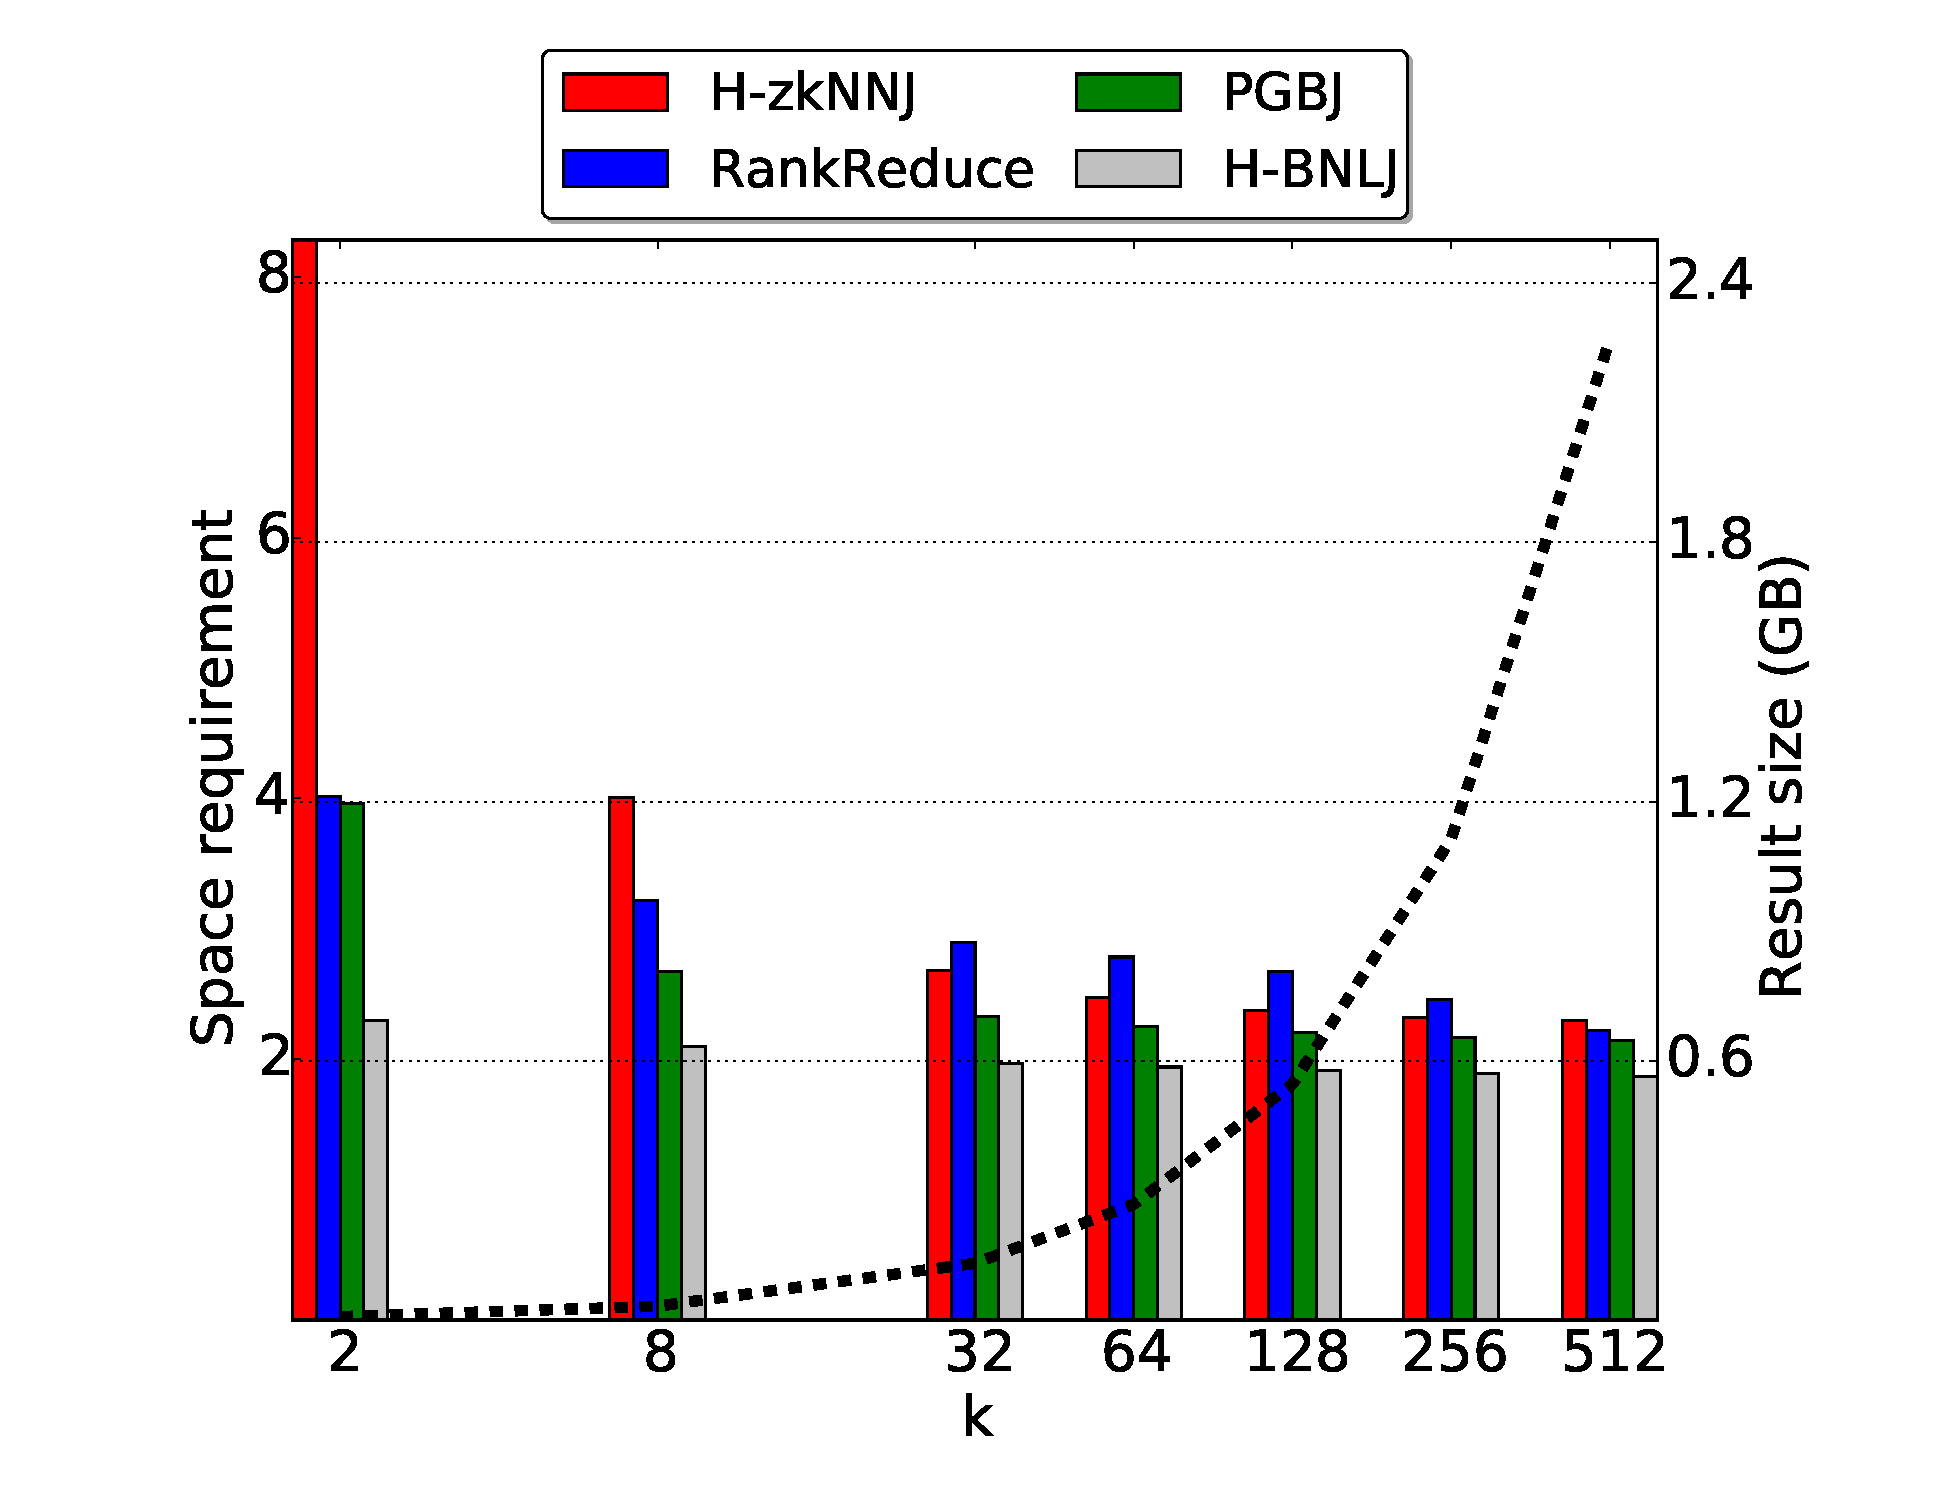
\includegraphics[width=\textwidth]{img-perf/geo/k/memory.pdf} 
		\caption{Result size and Disk Usage\label{fig:geo_k_memory} }
	\end{subfigure}%
	\begin{subfigure}[b]{0.35\textwidth}
		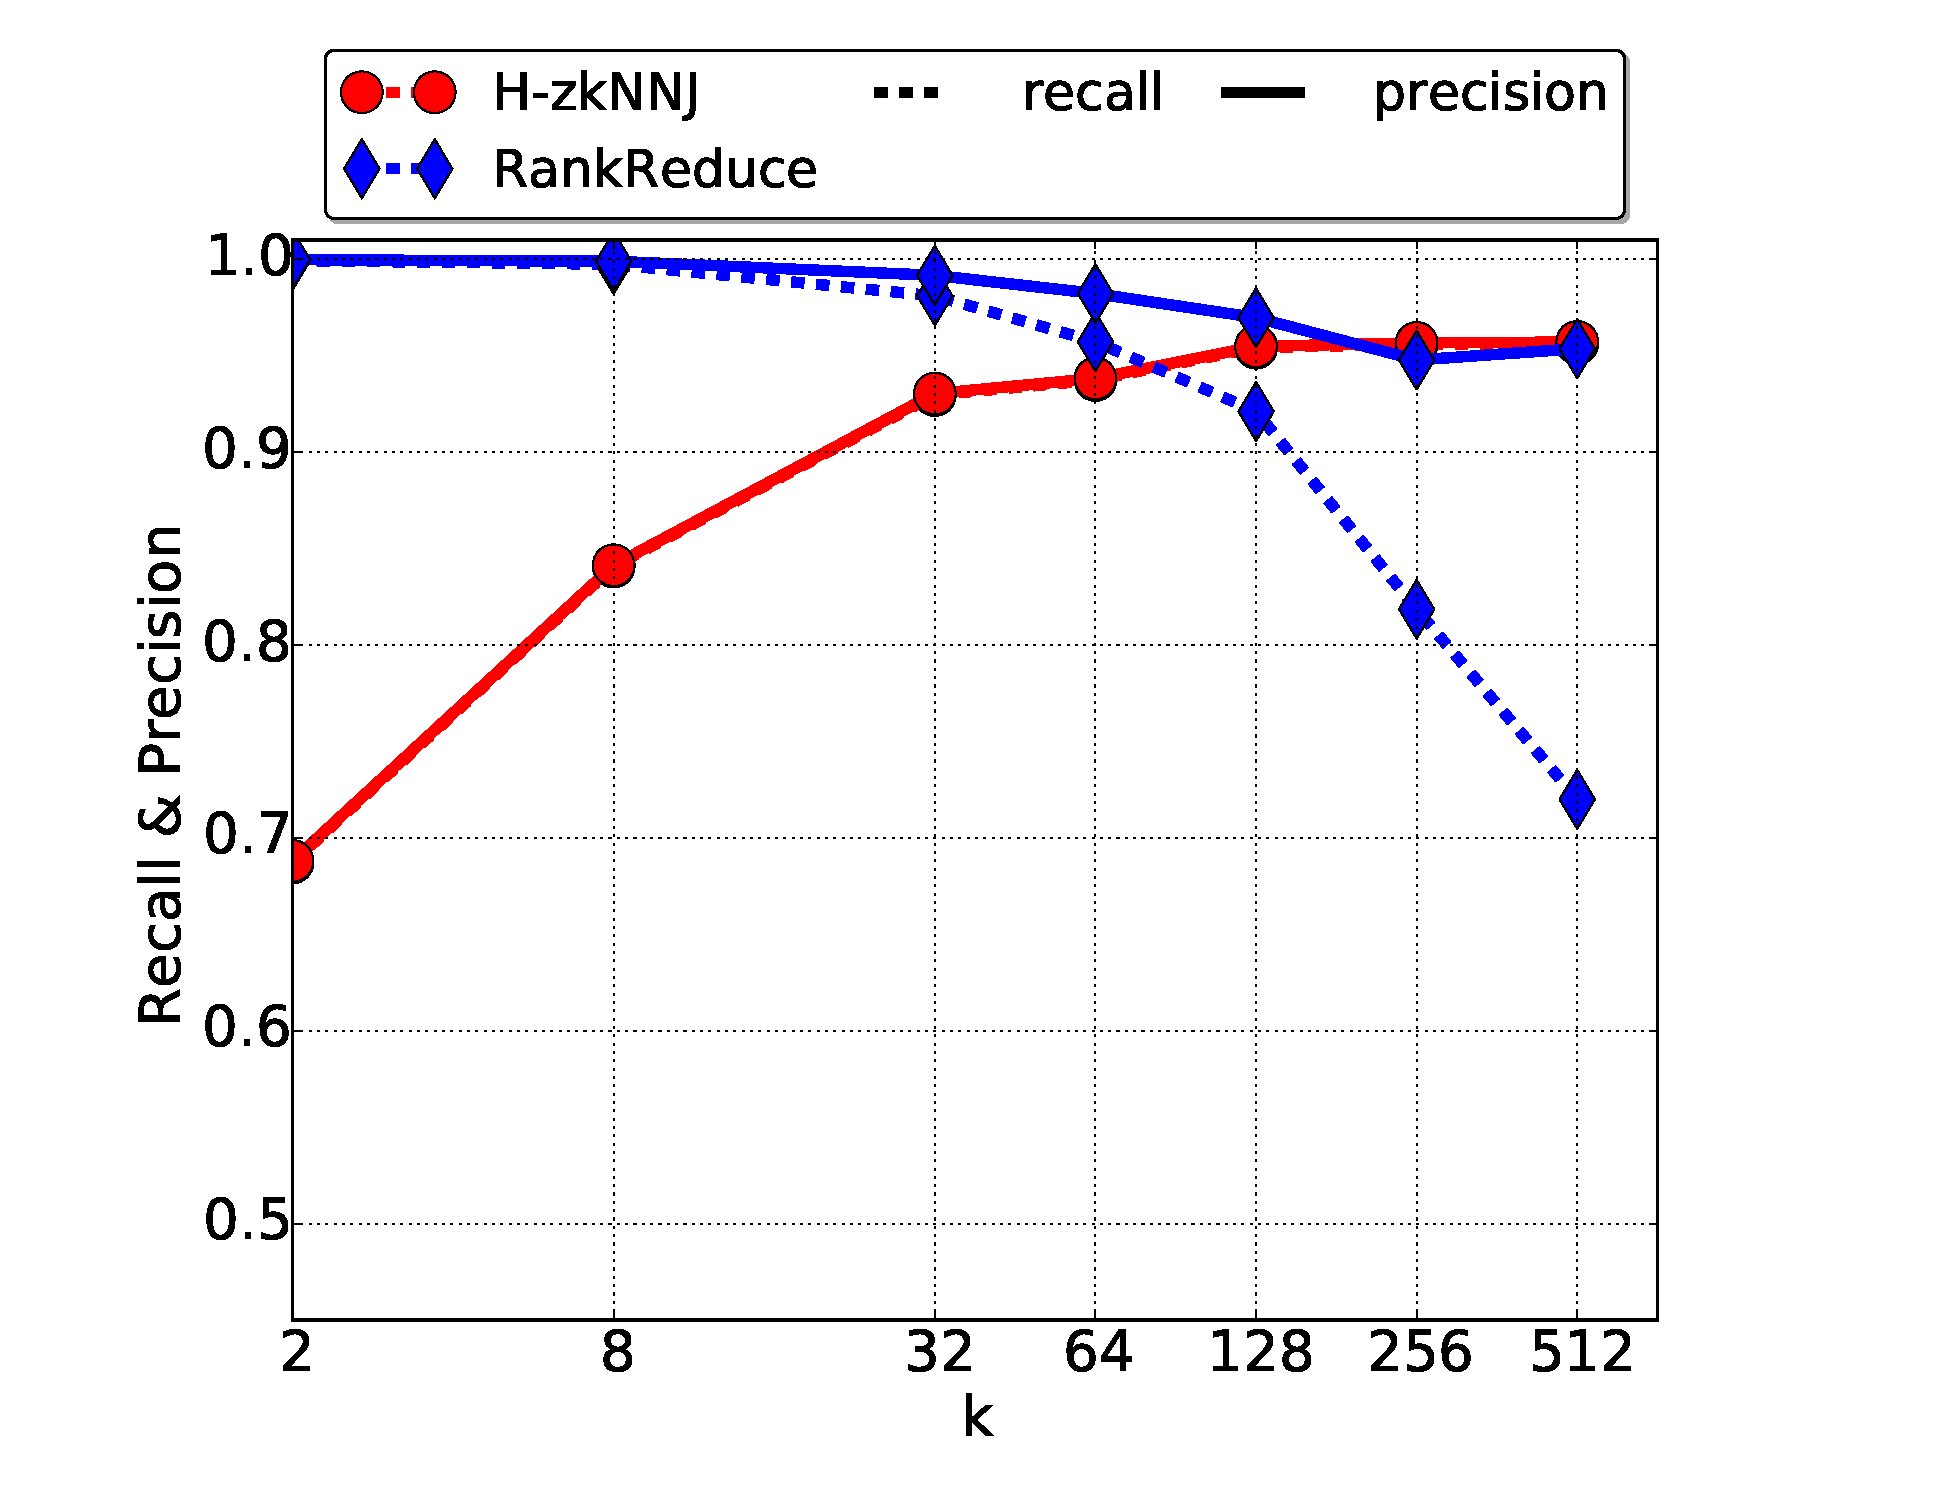
\includegraphics[width=\textwidth]{img-perf/geo/k/accuracy.pdf} 
		\caption{Recall and Precision \label{fig:geo_k_acc}}            
	\end{subfigure}%
	\caption{ Geo dataset with 200k records (50k for H-BNLJ), impact of $K$  }
	\label{fig:geo_impact_k}
\end{figure*}

Second, the algorithms can also be distinguished considering their disk usage, visible on 
Figure ~\ref{fig:geo_k_memory}. The global tendency is that the ratio of intermediate data size over the final data 
size decreases. This means that for each algorithm the final 
data size grows faster than the intermediate data size. As a consequence, there is no particular algorithm that 
suffers from such a bottleneck at this point.
\VO~is \ the most efficient from this aspect. Its replication of data occurs independently of the number of 
selected neighbors. Thus, increasing $k$ has a small impact on this algorithm, both in computing time and space 
requirements. On this figure, an interesting observation can also be made for \Z. For $k=2$, it has by far the 
largest disk
usage but becomes similar to the others for larger values. 
This is because \Z~creates a lot of intermediate data (copies of the initial dataset, vectors for the space 
filling curve, sampling...) irrespective of the value of $k$. As $k$ increases, so does the output size, mitigating the 
impact of these intermediate data. 

Surprisingly, changing $k$ has a different impact on the recall of the approximate kNN methods, as can be seen on 
Figure~\ref{fig:geo_k_acc}.
For \LSH, increasing $k$ has a negative impact on the recall which sharply decreases when $k\geq 64$. This is
because the window parameter ($W$) of LSH was set at the beginning of the experiments to achieve the best performance for this
particular dataset. However, it was not modified for various of $k$. Thus it became less optimal as $k$ increased. This 
shows there is a link between global parameters such 
as $k$ and parameters of the LSH process. When using \Z, 
increasing $k$  improves the precision: the probability to have incorrect points is reduced as there are more 
candidates in a single partition. 

\subsubsection{Communication Overhead}
Our last set of experiments looks at inter-node communication by measuring the amount of data transmitted during the
shuffle phase (Figure~\ref{fig:geo_communication}). The goal is to compare these measurements with the theoretical 
analysis in Section~\ref{section:global_complexity}, 

%%%% Generated with   2-time.py  and A4-ratioByK.py
\begin{figure*}[htp]
	\centering
	\begin{subfigure}[b]{0.48\textwidth}
		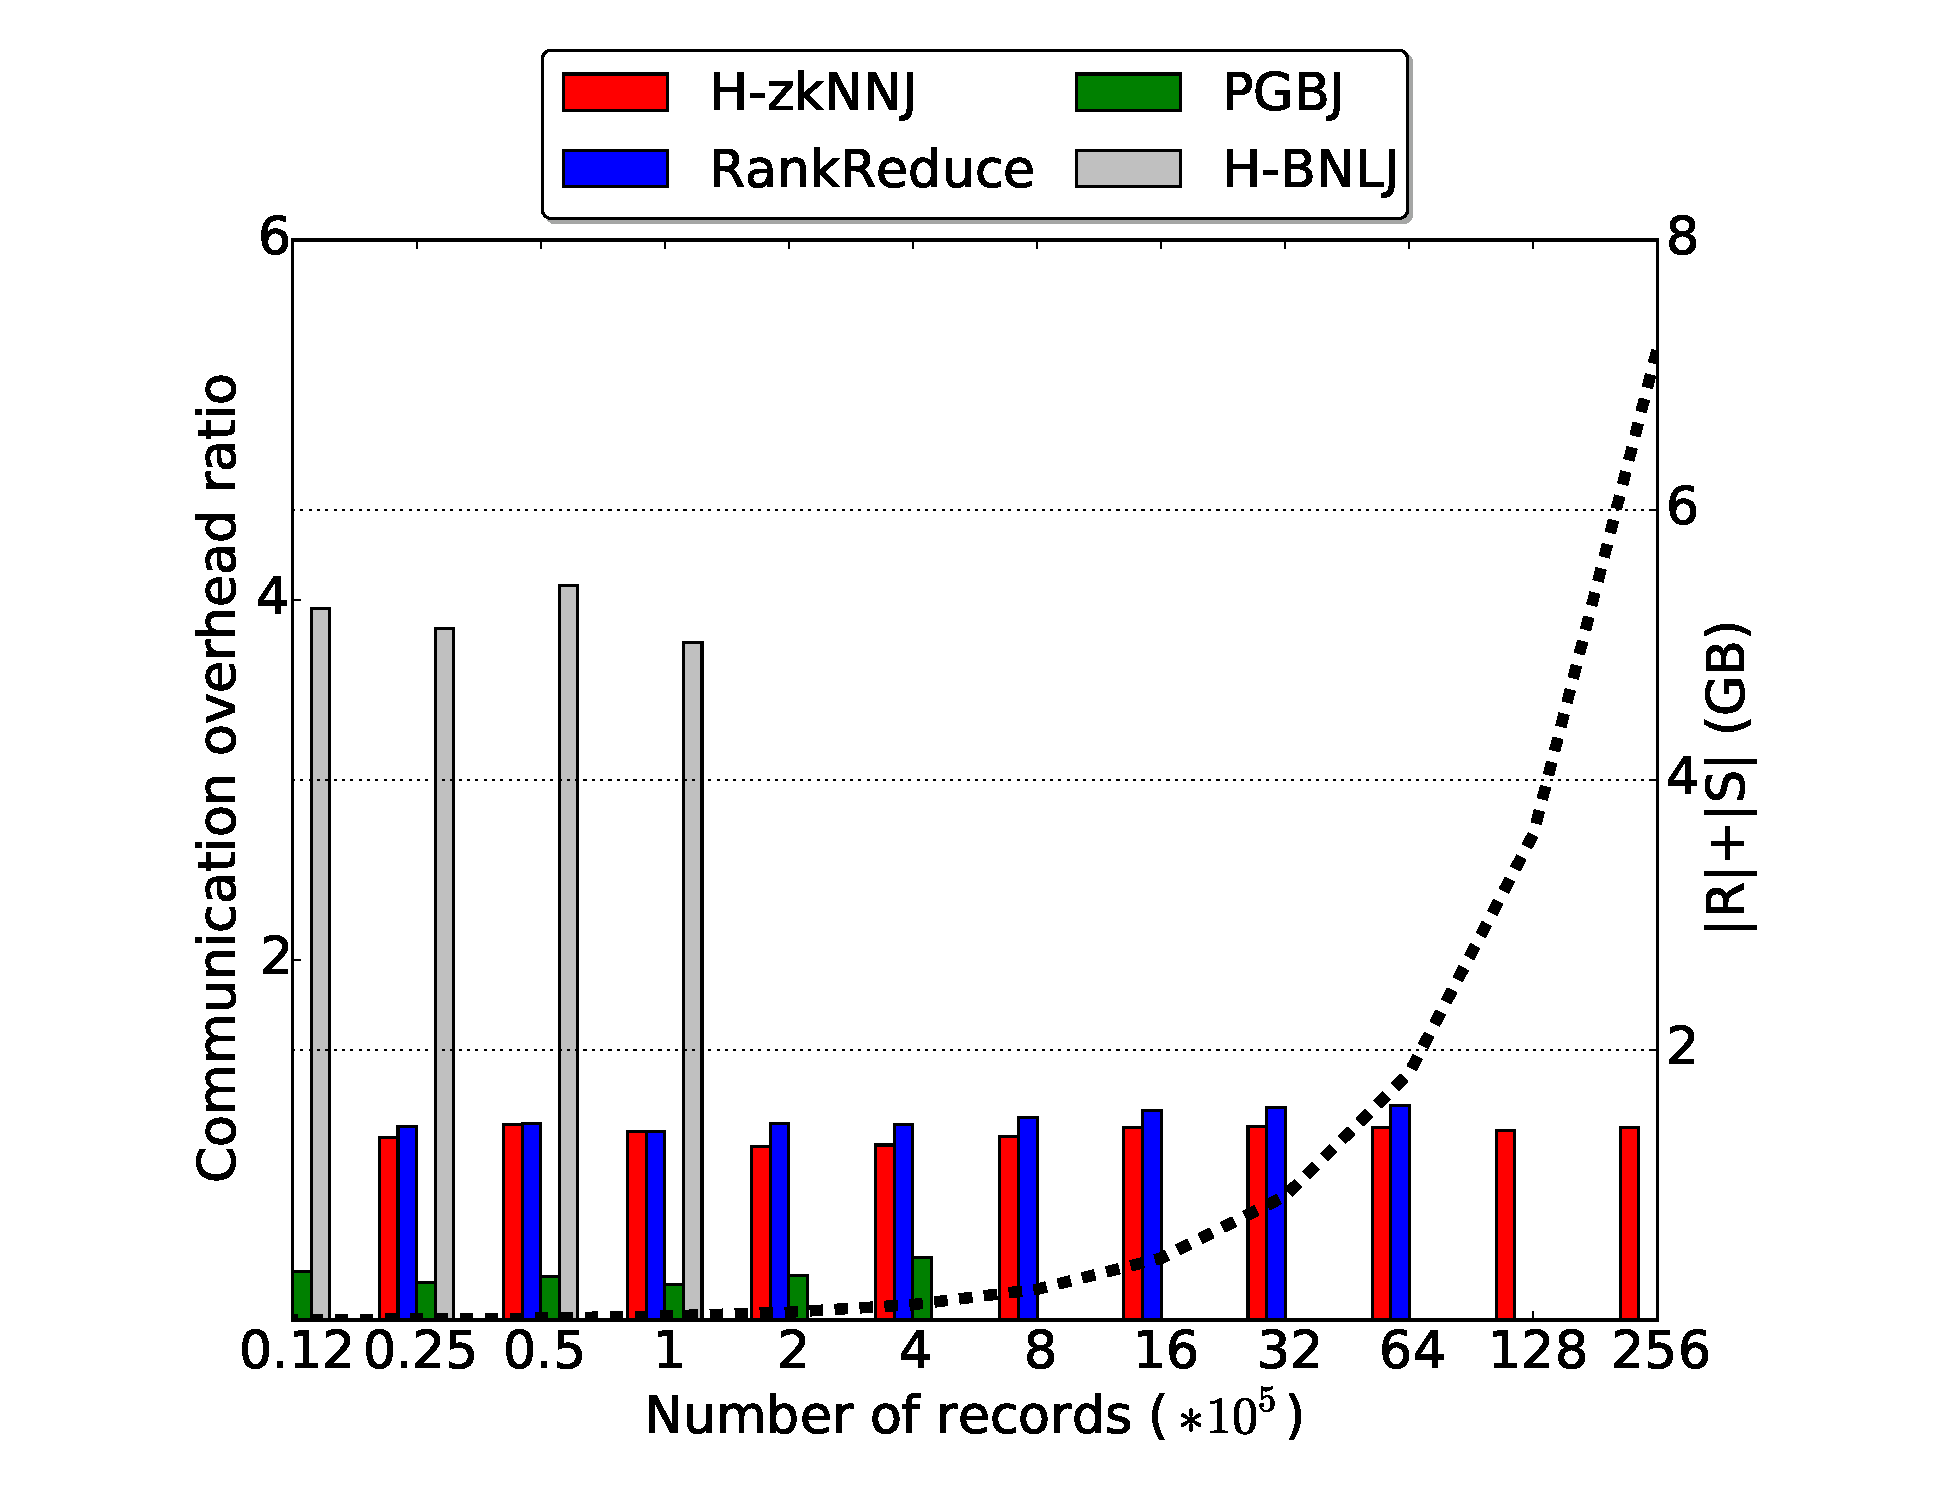
\includegraphics[width=\textwidth]{img-perf/geo/data/shuffle.pdf} 
		\caption{Impact of the data set size\label{fig:geo_data_shuffle}}
	\end{subfigure}%
	\begin{subfigure}[b]{0.48\textwidth}
		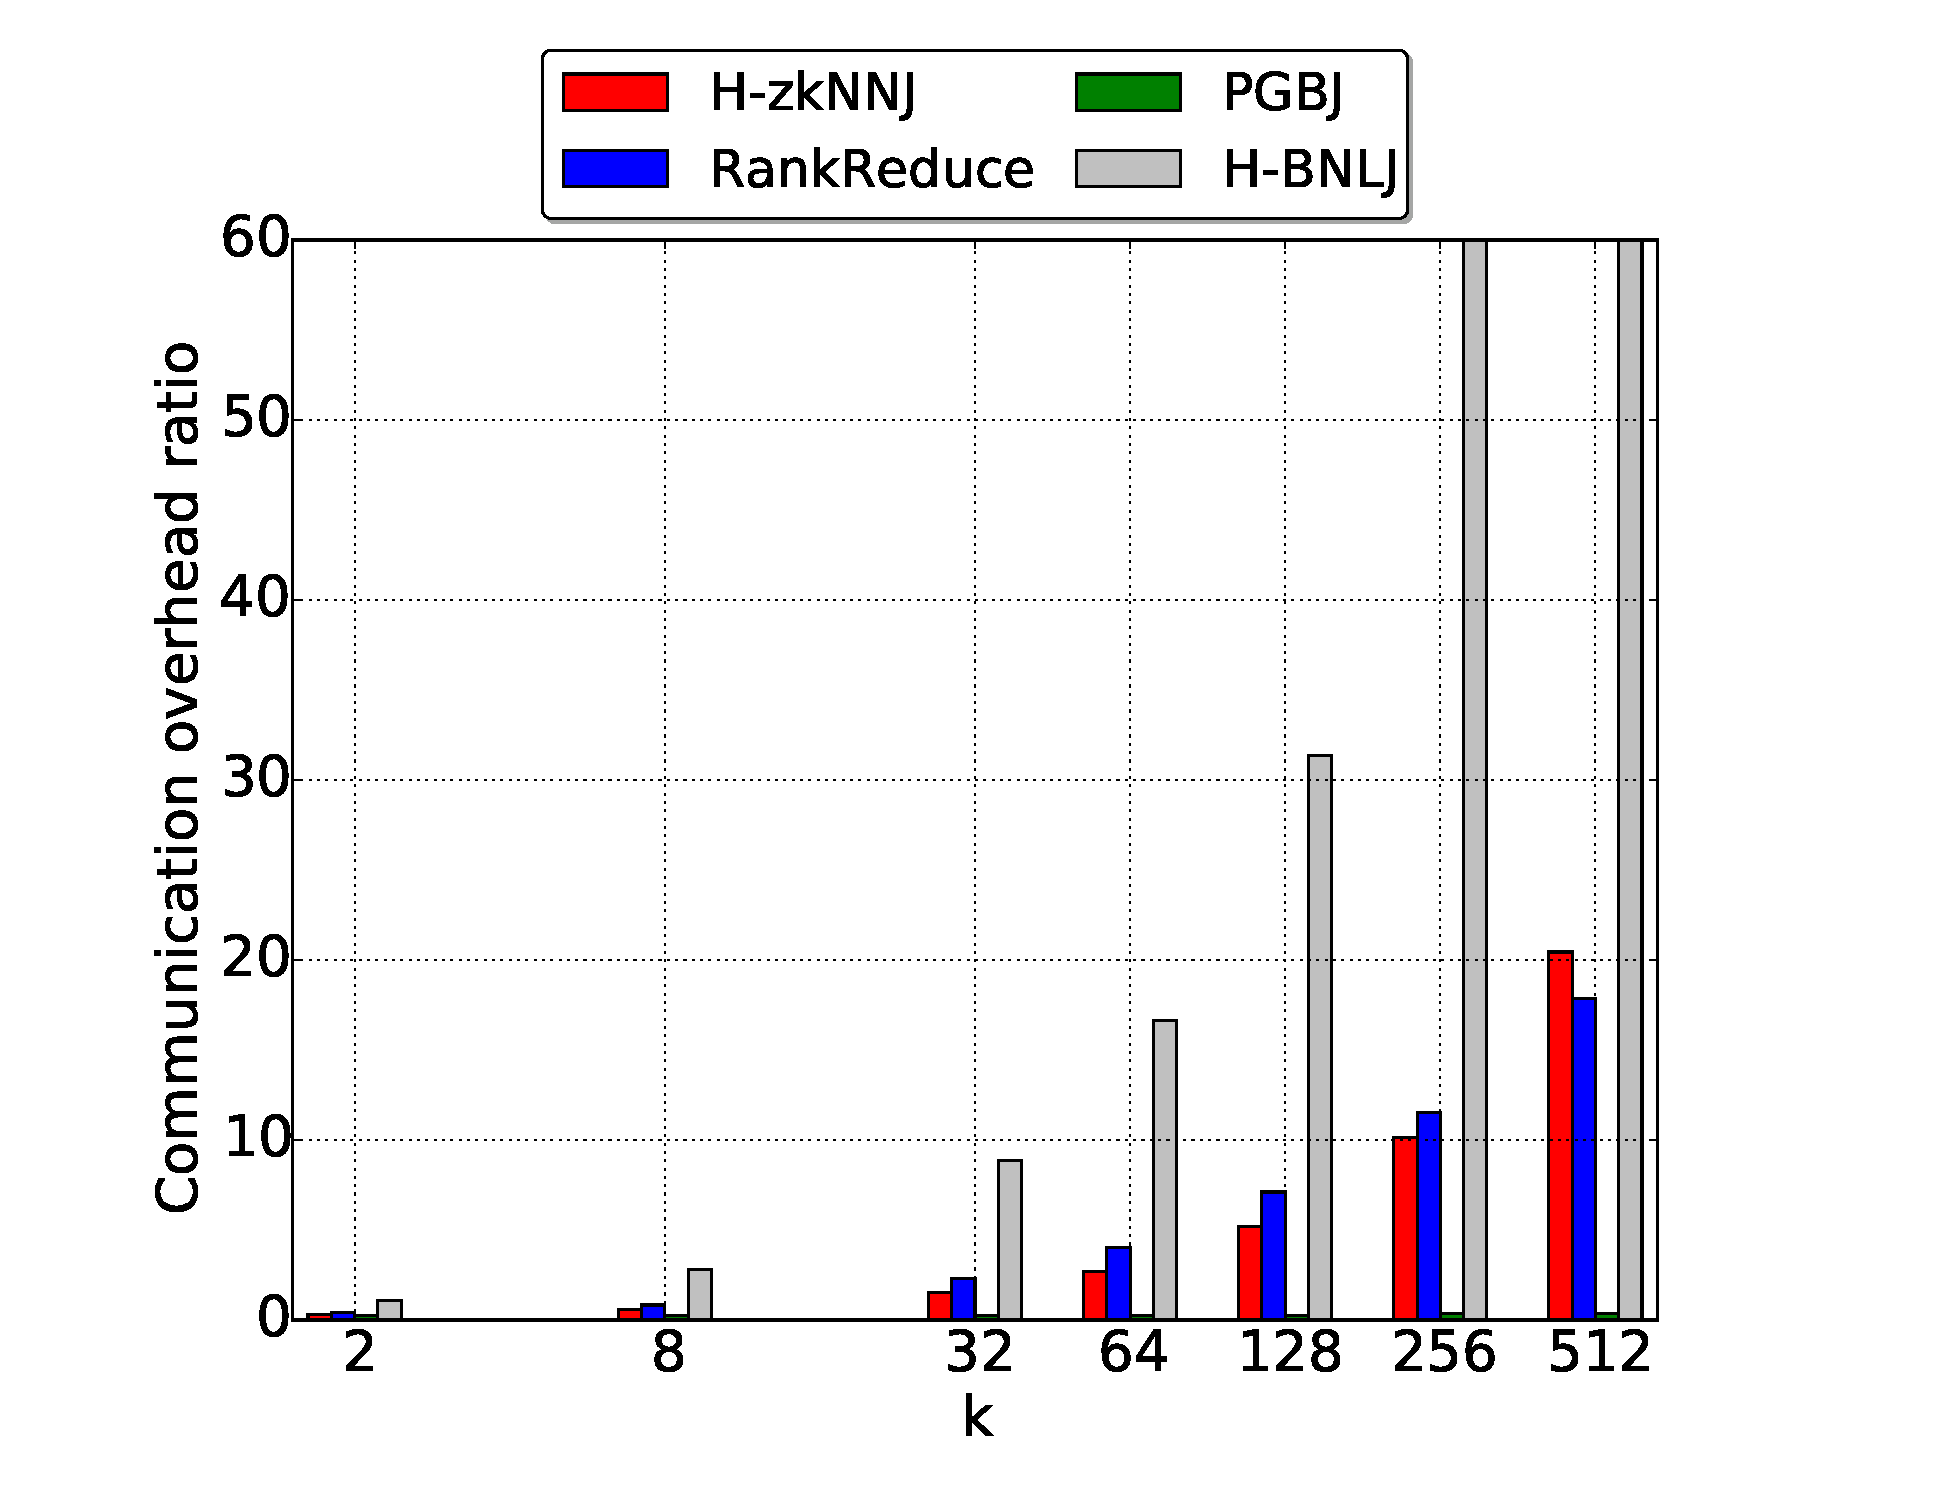
\includegraphics[width=\textwidth]{img-perf/geo/k/shuffle.pdf} 
		\caption{Impact of $K$ with $2*10^5$ records ($0.5*10^5$ for H-BNLJ) \label{fig:geo_k_shuffle}}
	\end{subfigure}%
	\caption{Geo dataset, communication overhead \label{fig:geo_communication}}      
\end{figure*}

\emph{Impact of data size.} For Geo dataset (Figure~\ref{fig:geo_data_shuffle}), \HBNLJ~has indeed a lot of 
communication. For a dataset of $1*10^5$ records, the shuffle phase transmits almost $4$ times the original size.
Both \LSH~and \Z~have a constant factor of $1$ because of the duplication of the original 
dataset
to improve the recall. The most efficient algorithm is \VO~for two reasons. First it does not duplicate the 
original dataset and second, it relies on various grouping strategies to minimize replication.

\emph{Impact of k.}
We have performed another set of experiments, with a fixed dataset of $2*10^5$ records (only $0.5*10^5$ for \HBNLJ). 
The results can be seen in Figure~\ref{fig:geo_k_shuffle}. For different values of $k$, we have a similar hierarchy 
than with the data size. For \LSH~and \Z, the shuffle increases linearly because the number of candidates in the second 
phase depends on $k$. Moreover \Z~also replicates $k$ previous and succeeding elements in the first phase, and because 
of that, its overhead becomes significant for large $k$. Finally in \VO, $k$ has no impact on the shuffle phase.
